%Imports and headers
\documentclass[a4paper]{article}  %Or use titlepage

%% For long tables in the appendix
\usepackage{longtable}

%% Language and font encodings
\usepackage[english]{babel}
\usepackage[utf8]{inputenc}
\usepackage[T1]{fontenc}
\usepackage{float} %makes you be able to use H option, places fig there and only there. VERY useful

%% Sets page size and margins
\usepackage[a4paper,top=3cm,bottom=2cm,left=3cm,right=3cm,marginparwidth=1.75cm]{geometry}

%% Useful packages for graphics and colors
\usepackage{amsmath}
\usepackage{graphicx, wrapfig}
\usepackage[colorinlistoftodos]{todonotes}
\usepackage[colorlinks=true, allcolors=blue]{hyperref}

%% Extra packages
\usepackage{geometry}
\usepackage{threeparttable}
\usepackage{xcolor}
\usepackage{amsmath}
\usepackage[some]{background}

%% Header, foot and page number in bottom right corner
\usepackage{fancyhdr}
\usepackage{lipsum}

%% For long comments
\usepackage{comment}
\usepackage{csquotes}

% nomenclature
\usepackage{nomencl}
\usepackage{booktabs}

% Turn on the style
\pagestyle{fancy}
% Clear the header and footer
\fancyhead{}
\renewcommand{\headrulewidth}{0pt}  % Remove head bar
\fancyfoot{}

% The file containing our references, in BibTeX format
\usepackage{csquotes} % Recommended by biblatex
\usepackage[style=numeric,sorting=none,backend=biber]{biblatex}
\addbibresource{references.bib}

%%%%% Title page
\begin{document}
\thispagestyle{empty}
\begin{titlepage}
\title{\vspace{60mm} \bf
        Containerization of microbial protoeomics data processing pipelines
}  %Fix to center title vertically
\author{Timothy Bergström}
\maketitle
\thispagestyle{fancy}  %Page number for title (\maketitle clears foot and head, so it needs to be after it)
\vspace*{\fill}
\centering{tib@kth.se \\ KTH: Royal institute of technology}
\end{titlepage}

\newpage

%%%%% Abstract
\begin{center}\normalfont\Large\bfseries\centering Abstract\end{center}
NOT WRITTEN YET

\newpage

\begin{center}\normalfont\Large\bfseries\centering Referat\end{center}
INTE SKRIVEN ÄN

\newpage

%%%%% Table of contents
\thispagestyle{empty}
\tableofcontents
\newpage

%%%% Nomenclature
\makenomenclature
%ABCDEFGHIJKLMNOPQRSTUVXYZ
\nomenclature{$CID$}{Collision Induced Dissociation}
\nomenclature{$FDR$}{False Discovery Rate}
\nomenclature{$GUI$}{Graphical User Interface}
\nomenclature{$HPC$}{High Performance Computing}
\nomenclature{$LC$}{Liquid Chromatography}
\nomenclature{$LFQ$}{Label-Free Quantification}
\nomenclature{$MS$}{Mass Spectrometry}
\nomenclature{$OS$}{Operative System}
\nomenclature{$POSIX$}{Portable Operating System Interface}
\nomenclature{$PSM$}{Peptide to Spectrum Matches}
\nomenclature{$VM$}{Virtual Machine}

\printnomenclature
\newpage

%%%%% Chapters
% set footer
% Set the right side of the footer to be the page number
\fancyfoot[R]{\thepage}  % Page number
\fancyfoot[L]{\date{\today}}  % date on footer
\setcounter{page}{1}

\section{Introduction}

Mass spectrometry (MS)-based Proteomics is currently the most comprehensive technique to analyze protein content in biological samples. Modern MS generate vast amounts of data and the analysis of such data is generally considered as a bottleneck, both due to the volume of data but also as the methods for processing the data are complex and need manual intervention. As it is hard to recreate the exact software environment used during processing, the majority of all results produced with mass spectrometers cannot be accurately reproduced outside of the lab where it was initially generated.

Containerization and workflow management is a way to remedy the situation. Containerization is a technique to install software, not into a particular computer, but into a virtual container environment, in a so-called image. The image can be distributed to several separate computers, yet guaranteed to execute in the exact same way regardless of the operating system. There are several such containerization techniques available. Here, we will focus on one named Singularity, as it is the preferred solution of most HPC clusters, such as UPPMAX.

The second concept, workflow management, deals with how different pieces of dependent software can be consequently executed in a particular environment. Again, there are several workflow managers available, but we will focus on one named NextFlow as it currently is a preferred solution for sequencing data at SciLifeLab.

The aim of the project is to utilize containerization to embed a software named \textit{Quandenser}, a newly created software made in SciLifeLab by Lukas Käll and Matthew The, which condenses quantification data from label-free MS experiments \cite{quandenser}. In unison with several other software embedded in the container, a workflow is to be created based on Nextflow with the aim to analyze MS generated data to protein quantification results.

\section{Method}

\subsection{The singularity image}
A Singularity image needs a so called "receipt", which is a file that tells Singularity how to create the image and what to include in it. The recipe was added to Singularity Hub, an online library were Singularity receipts can be uploaded, which are then automatically built, so they can shared with other users \cite{singularity-hub}.

To complete the workflow from raw data to protein quantification results, several other software had to be included in the container, which are listed below.

\subsection{Quandenser} \label{ssec:quandenser-method}
 The core component in Quandenser-pipeline is Quandenser, which is a newly created software made in the lab of Statistical Biology at SciLifeLab, which condenses quantification data from label-free MS experiments by clustering both data from MS1 and MS2 without assigning identities to the values, thus decouples identification from quantification \cite{quandenser}. Due to Quandenser-pipeline can be run on clusters where singularity is installed (which is the case for UPPMAX), it opens up the possibility for parallelization, a method to speed up the processing time of software.

A modified version of Quandenser was added to the pipeline, which can utilize parallel computation in conjunction with Nextflow's ability to run multiple processes in parallel. The improvements were integrated into the internal pipeline of Quandenser, which is shown in figure \ref{fig:quandenser-internal-pipeline}.

\begin{figure}[H]
  \centering
  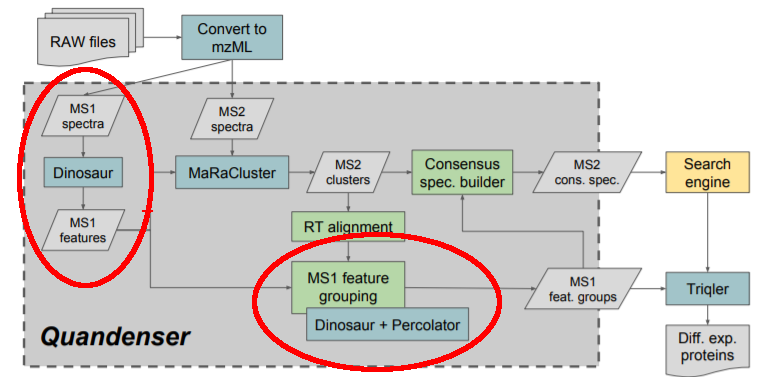
\includegraphics[width=\linewidth]{pictures/quandenser-internal.png}
  \caption{\textbf{The internal pipeline of Quandenser (image from The M. and Käll L. \cite{quandenser})}. Processes highlighted in red circles was modified to integrate the parallelization of Quandenser}
  \label{fig:quandenser-internal-pipeline}
\end{figure}

Two parts were able to be parallelized within Quandenser's internal pipeline, highlighted in figure \ref{fig:quandenser-internal-pipeline}. The parallelization was done by adding "stop points" in Quandenser's code to allow Nextflow to run part of the pipeline in parallel, spawning a new process of Quandenser for each process. The first parallelizable part was "MS1 feature detection" with the internal program \textit{Dinosaur}, shown in figure \ref{fig:quandenser-internal-pipeline}. This is the first step in Quandenser's internal pipeline and was able to be "fully" parallelized, meaning that every process can be processed in parallel. The second part which was able to be parallelized was "MS1 feature grouping", shown in figure \ref{fig:quandenser-internal-pipeline}. This could only be partially parallelized, due to the input files are calculated in a minimum spanning tree, a way to minimize the amount of connections and weights in a tree \cite{min-span-tree}. An explination of why the process could not be fully parallelized is that connecting branches cannot be calculated at the same time, while branches that are not directly connected can be processed in parallel. To cluster and process all files, the files must be calculated in a particular order according to the tree, while the Nextflow pipeline utilizes the minimum spanning tree output from Quandenser to create a processing tree that maximizes the amount of files that can be processed in parallel, given the structure of the minimum spanning tree given by Quandenser.

\subsubsection{MSconvert}
There exist a multitude of different types of MS data format, which can cause compatibility issues with existing software. The MS format depends on which instrument was used to generate the data, but most software cannot directly use any vendor-specific formatted files directly. The solution is to convert files to a general MS data format first, most commonly files of type mzML \cite{mzml-format}. To combat the problem with incompatible data in the pipeline, a software named \textit{MSconvert} was added to the workflow, which can convert MS data from a multitude of vendor formats to the general MS data format needed to run Quandenser \cite{proteowizard}. Due to conversion from vendor formats with Msconvert only works on Windows operative systems, another solution was needed, since the Singularity image was based on Ubuntu, a Linux operative system. The solution was to use another type of software called \textit{Wine}, which adds an compatibility layer in Portable Operating System Interface (POSIX) systems, to run Windows software \cite{wine}. The Singularity image was based on another image created by the proteowizard developers, which incorporates all the necessary components to run Wine and MSconvert \cite{docker-image} \cite{docker-howto}.

\subsubsection{Crux}
Crux is an open source mass spectrometry analysis toolkit available for Linux, Windows and MacOS \cite{crux}. The purpose of integrating Crux into the image was to use three specific tools; tide-index, tide-search and percolator. Tide-index is a pre-search tool that adds indexes and decoys to the protein data base, which is used by the search tool tide-search, that parses fragmentation spectra and creates peptide-to-spectrum matches (PSMs) \cite{tide-search}. Percolator is a post-search tool, that separates peptide targets from decoy PSMs \cite{percolator}. In combination, the tools were used to post-process the output from Quandenser to prepare it for the software Triqler, another tool included in the image which is explained in the next section.

\subsubsection{Triqler}
Triqler is an software which uses using graphical models and bayesian statistics to find differentially expressed proteins between samples \cite{triqler}. Triqler can utilize MS2 and MS1 spectra from the Quandenser output with minor reformatting, meaning Triqler was an excellent tool to include in the image. However, the main benefit of using Triqler is the way it handles error propagation of quantification.

False Discovery Rate (FDR) is a statistical measurement of how many false positives there will be among positive results \cite{fdr}.  Triqler explicitly propagates uncertainty in the quantification process, meaning the FDR can be controlled and can be used to filter the quantifications at the end of the quantification process, which typical Label-free quantification (LFQ) pipeline fails to achieve \cite{triqler}. Futhermore, Triqler imputes missing values in a bayesian way by assigning a probability distribution over possible values of the missing values, with the uncertainty propagation explained above included. The missing value is then assigned by integrating the probability distributions over the possible imputed values, meaning the missing value is estimated more accurately compared to filling in the missing value with another, such as replacing it with the mean value \cite{triqler}.

\subsection{Nextflow}
Nextflow has integrated compatibility with running software inside Singularity images, meaning Nextflow can call on the programs contained within the Singularity image without any additional software. The pipeline of Quandenser-pipeline is shown in figure \ref{fig:workflow}. As explained in section \ref{ssec:quandenser-method}, Nextflow's capability of running multiple processes in parallel was use with a modified version of Quandenser to allow for paralellization. When running the parallelized version of Quandenser in the pipeline, the processes are divided into five parts, two of which are parallelizable. The aim was to speed up the calculation time when running large cohorts.

Nextflow also has the benefit of being able to submit processes to workload managers, which are used on HPC clusters to allocate processing time for users. To be able to run the pipeline on HPC clusters, the pipeline is outfitted with an option to enable submitting processes via SLURM, the current workload manager on UPPMAX.

\begin{figure}[H]
  \begin{center}
  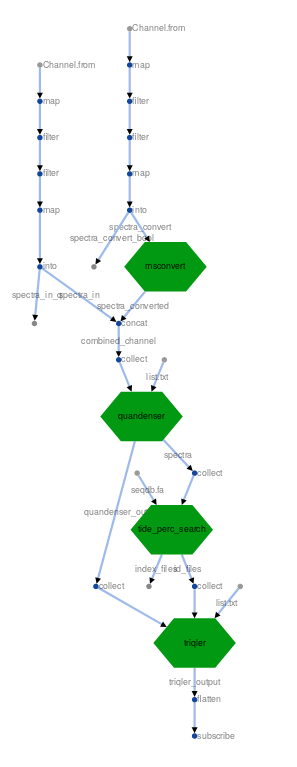
\includegraphics[width=0.5\linewidth]{pictures/workflow.png}
  \caption{\textbf{Workflow of the pipeline.} The node \textit{Batch file} in the workflow is a file containing paths to the mzML files and labels of the files to signify replicates}
  \label{fig:workflow}
  \end{center}
\end{figure}

\subsection{Quandenser-pipeline Graphical User Interface (GUI)}
To integrate the Singularity image and the Nextflow pipeline, a GUI was created and packed into the image to improve the usability of the workflow, to allow users to easily modify and run the pipeline to their choosing. Pyside2 was used to create the GUI, which is an open source GUI framework based by the Qt framework \cite{pyside2}. Figure \ref{fig:GUI} illustrates how the GUI looks like and shows how different types of files (vendor specific files and mzML), can be used in the same pipeline without any need to convert the files beforehand.

\begin{figure}[H]
  \begin{center}
  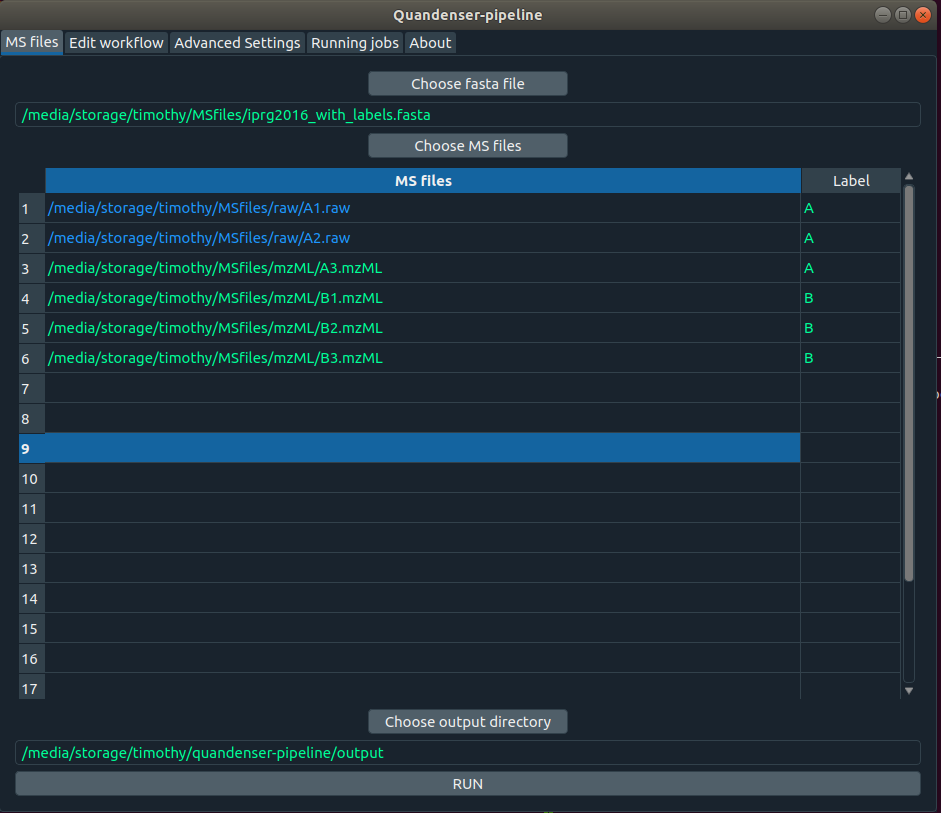
\includegraphics[height=7cm]{pictures/gui.png}
  \caption{\textbf{GUI of Quandenser-pipeline}. The user can choose any type of MS files to run through the pipeline, since the files will be converted before they enter Quandenser. The files which will be converted are highlighted in blue}
  \label{fig:GUI}
  \end{center}
\end{figure}

To allow users to easily download and run the GUI from within the image, a shell script was created to minimize manual intervention and installation. The shell script will install Singularity, downloading the image from Singularity Hub and start the GUI embedded inside the image. The GUI will then be used to modify the configurations for the pipeline, which affects how the pipeline is executed, by utilizing "named pipe", i.e. a file which both the GUI and the shell script has access to. If the user executes the program, the GUI tells the shell script to execute the Nextflow pipeline by modifying the values inside the named named pipe. The Nextflow pipeline then runs the Singularity image and executes the embedded software in the image at a particular order.

\subsection{Benchmark on bacterial proteomic data}
The two data sets were generated in Paul Hudson's lab at SciLifeLab. The first data set was generated by letting cyanobacteria grow in five different simulated environments (before sunrise, after sunrise, noon, before sunset and after sunset) with two replicates each, resulting in a total of 10 files. The second bacterial data set was ralstonia bacteria being grown in a chemostat bioreactor where Formic Acid (FA) was limited during the experiment, in five different conditions (0.05, 0.10, 0.15, 0.20 and 0.25 growth-rate) with four replicates each, resulting in a total of 20 files.

The RAW data files for the cyanobacteria data set and ralstonia data set was on average 0.8 Gb respectively 1.3 Gb in size. Both data sets were run on different established proteomic pipelines to compare the performance of the newly created pipeline.

Two other pipelines using non-container software were tested on the bacterial proteome data. The following table illustrates which pipelines were used:

\newcommand{\textone}{\small The pipeline created for the thesis, using Quandenser as it's cornerstone. Due to Singularity not supporting non-POSIX systems, the Windows OS cannot run the pipeline natively without using a compatibility layer. An virtual machine wrapper was developed to allow users to run the pipeline in Windows}
\newcommand{\texttwo}{\small The custom pipeline tested on the data set was created by the workflow manager \textit{KNIME} in combination with \textit{OpenMS}, creating a custom workflow for analyzing mzML data \cite{knime} \cite{openms}. The pipeline was created by Michael Jahn at Paul Hudson's lab in SciLifeLab and was used to analyze bacterial data \cite{m-jahn-pipeline}. Both KNIME and OpenMS is available for Linux, MacOS and Windows.}
\newcommand{\textthree}{\small MaxQuant is a tool used for quantitative proteomics and is well suited for analyzing label-free proteomic data. The program can be run natively on Windows and on Linux with the framework \textit{Mono} \cite{maxquant} \cite{maxquant-installation}.}

\begin{table}[H]
\caption{\textbf{Different pipelines used to compare Quandenser-pipeline}}
\begin{center}
\begin{tabular}{|p{4cm}|p{9cm}|}
\hline
Program & Description \\ \hline \hline
Quandenser-pipeline v0.071 & \textone \\ \hline
KNIME + OpenMS & \texttwo \\ \hline
MaxQuant 1.6.3.3 & \textthree \\ \hline
\end{tabular}
\end{center}
\end{table}

\subsubsection{Finding differentially expressed proteins}
Significantly differentially expressed proteins were also analyzed from the cyanobacteria data set with the output from Quandenser-pipeline. To define a differentially expressed protein, a relevant statistical parameter was chosen to represent how statistically significant find is; the q-value. A q-value is an excellent statistical measurement when doing multiple tests, which in this case is for each specific protein \cite{q-value}.

The threshold of a differentially expressed protein was set as a q-value less than 0.05. In contrary to the p-value, a p-value threshold of 0.05 means 5\% of all tests will result in a false positives while a q-value threshold of 0.05 will result in 5\% of all \textit{significant} differentially expressed results being false positives \cite{q-value} \cite{nonlinear}. Triqler, a tool included in the pipeline, automatically calculates q-values of proteins and only proteins under the q-value threshold of 0.05 was considered as "differentially expressed".

\section{Results}

\subsection{Pipeline performances}

The programs were run on a computer with an Intel Core i7-4790k CPU @ 4.0 GHz with 32 Gb of memory. The following histogram show the processing time of Quandenser pipeline, OpenMS and MaxQuant for the two data sets.

\begin{figure}[H]
  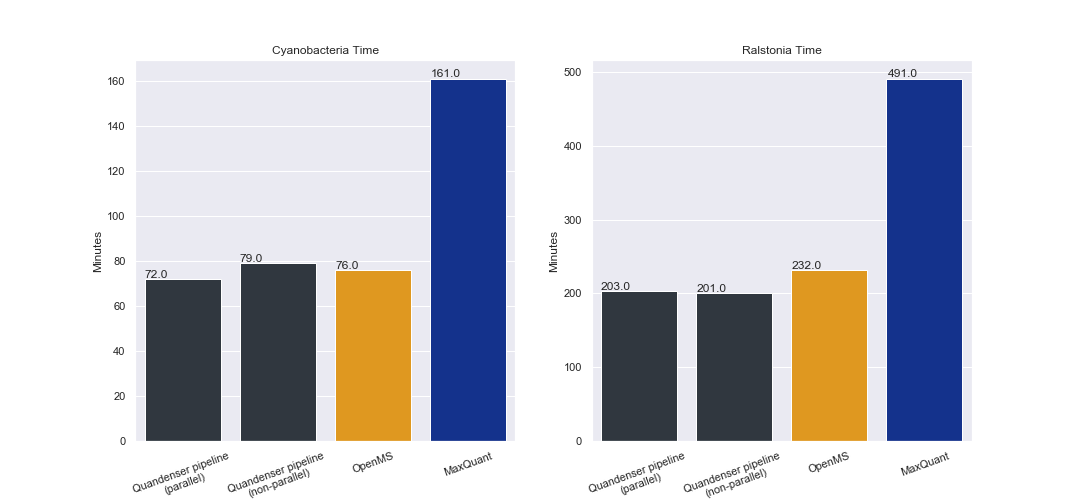
\includegraphics[width=\linewidth]{results/times.png}
  \caption{\textbf{Processing time on local computer (wall time)}. QP is the newly created pipeline and the y-axis of the plots shows the wall time (i.e. the processing time) of the different pipelines. Lower means less time to complete the process. The plot at the left illustrates the processing time of the cyanobacterial data set (10 files, about 0.8 Gb each), while the plot at the right is the processing time of the ralstonia data set (20 files, about 1.3 Gb each). Note that \textit{parallel} Quandenser used a maximum of two forks (aka two processes in parallel), which was the maximum the computer could handle}
  \label{fig:processing-local}
\end{figure}

\begin{figure}[H]
  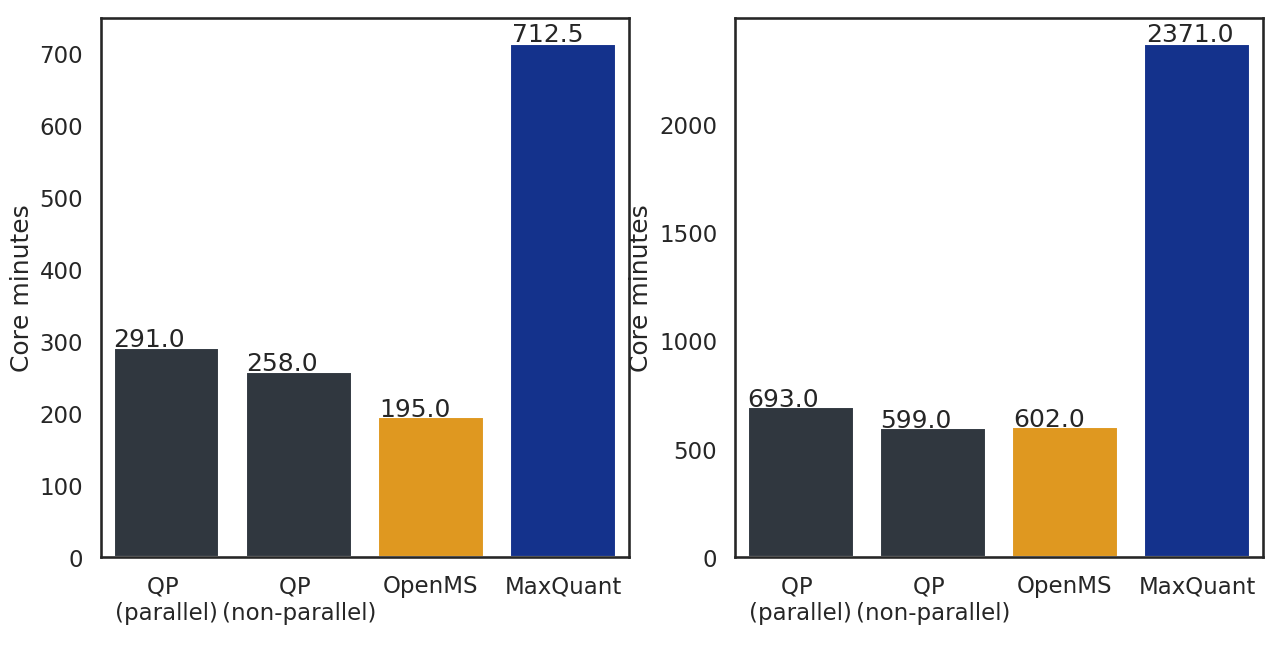
\includegraphics[width=\linewidth]{results/times_core.png}
  \caption{\textbf{Core minutes to finish process on local computer}. The y-axis of the plots shows core minutes used (i.e. how much the computer resources used) of the different pipelines. Lower means less computational resources used to finish the process. The plot at the left illustrates the core minutes used to process the cyanobacterial data set (10 files, about 0.8 Gb each), while the plot at the right is the core minutes used to process the ralstonia data set (20 files, about 1.3 Gb each). Note that \textit{parallel} Quandenser used a maximum of two forks (aka two processes in parallel), which was the maximum the computer could handle}
  \label{fig:processing-local-cores}
\end{figure}


\begin{figure}[H]
  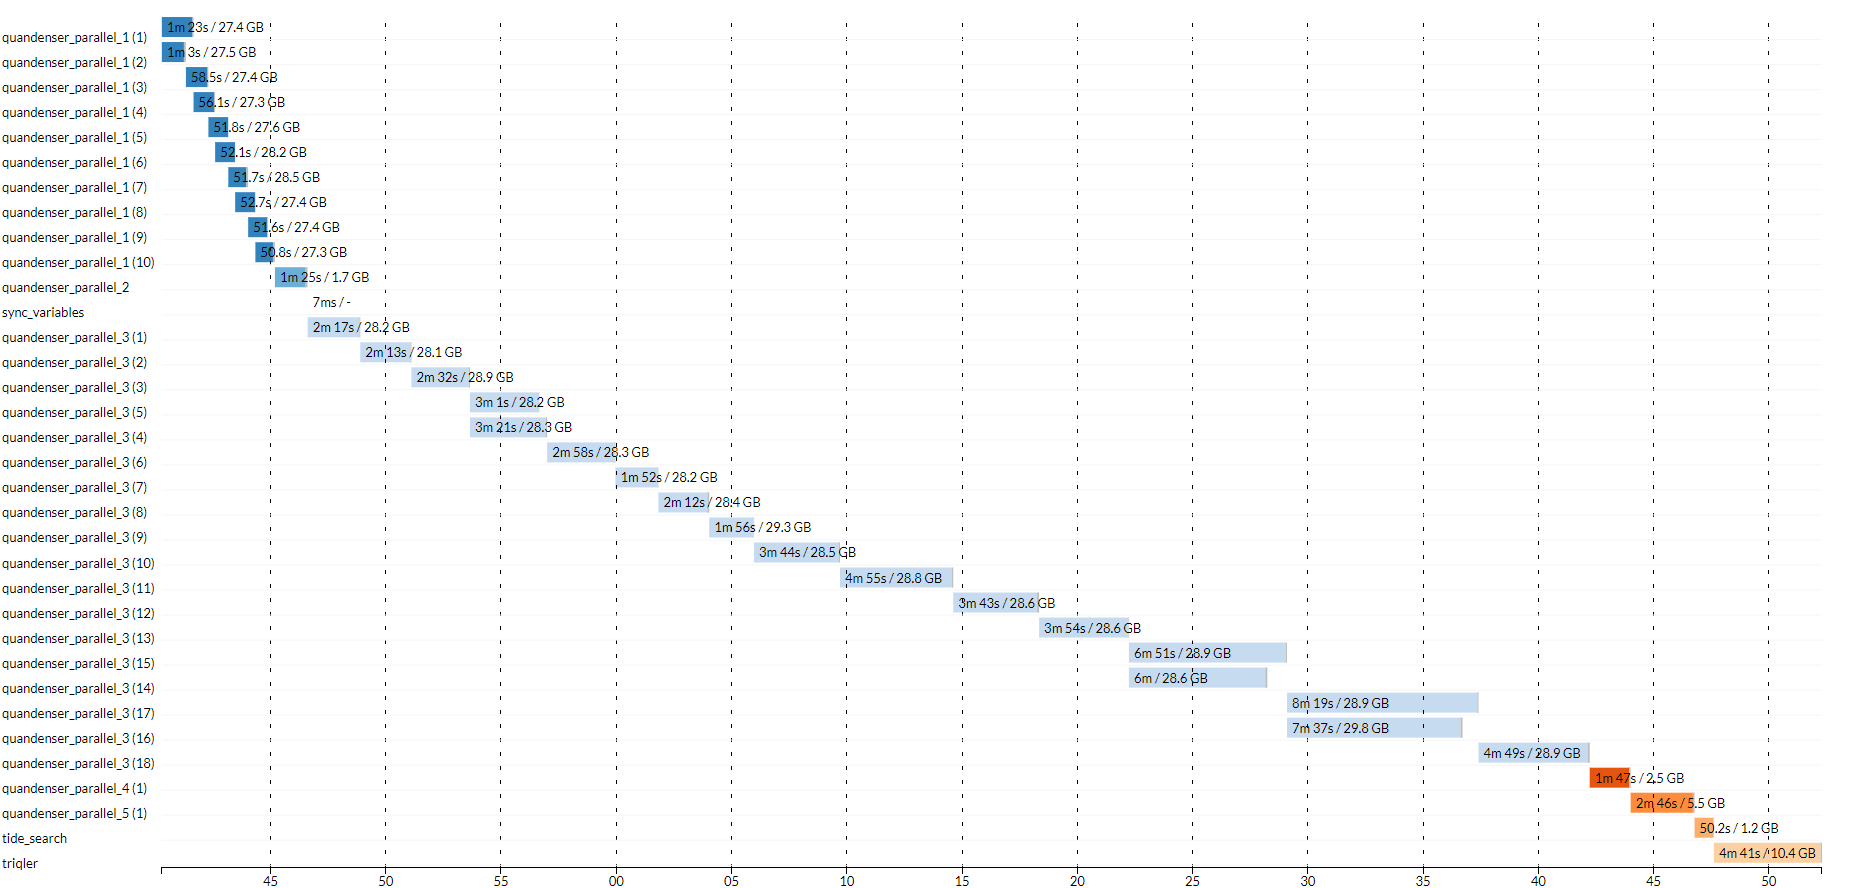
\includegraphics[width=\linewidth]{results/timeline-local.png}
  \caption{\textbf{Timeline of parallel processing of the cyanobacteria data set on the local computer.} Note that \textit{quandenser\_parallel\_1} is "fully" parallelizable while \textit{quandenser\_parallel\_3} is partially parallelized, following a minimum spanning tree explained in section \ref{ssec:quandenser-method}. The rest of the processes are non-parallelizable. A maximum of two forks was set (aka two processes in parallel)}
  \label{fig:timeline-local}
\end{figure}

\begin{figure}[H]
  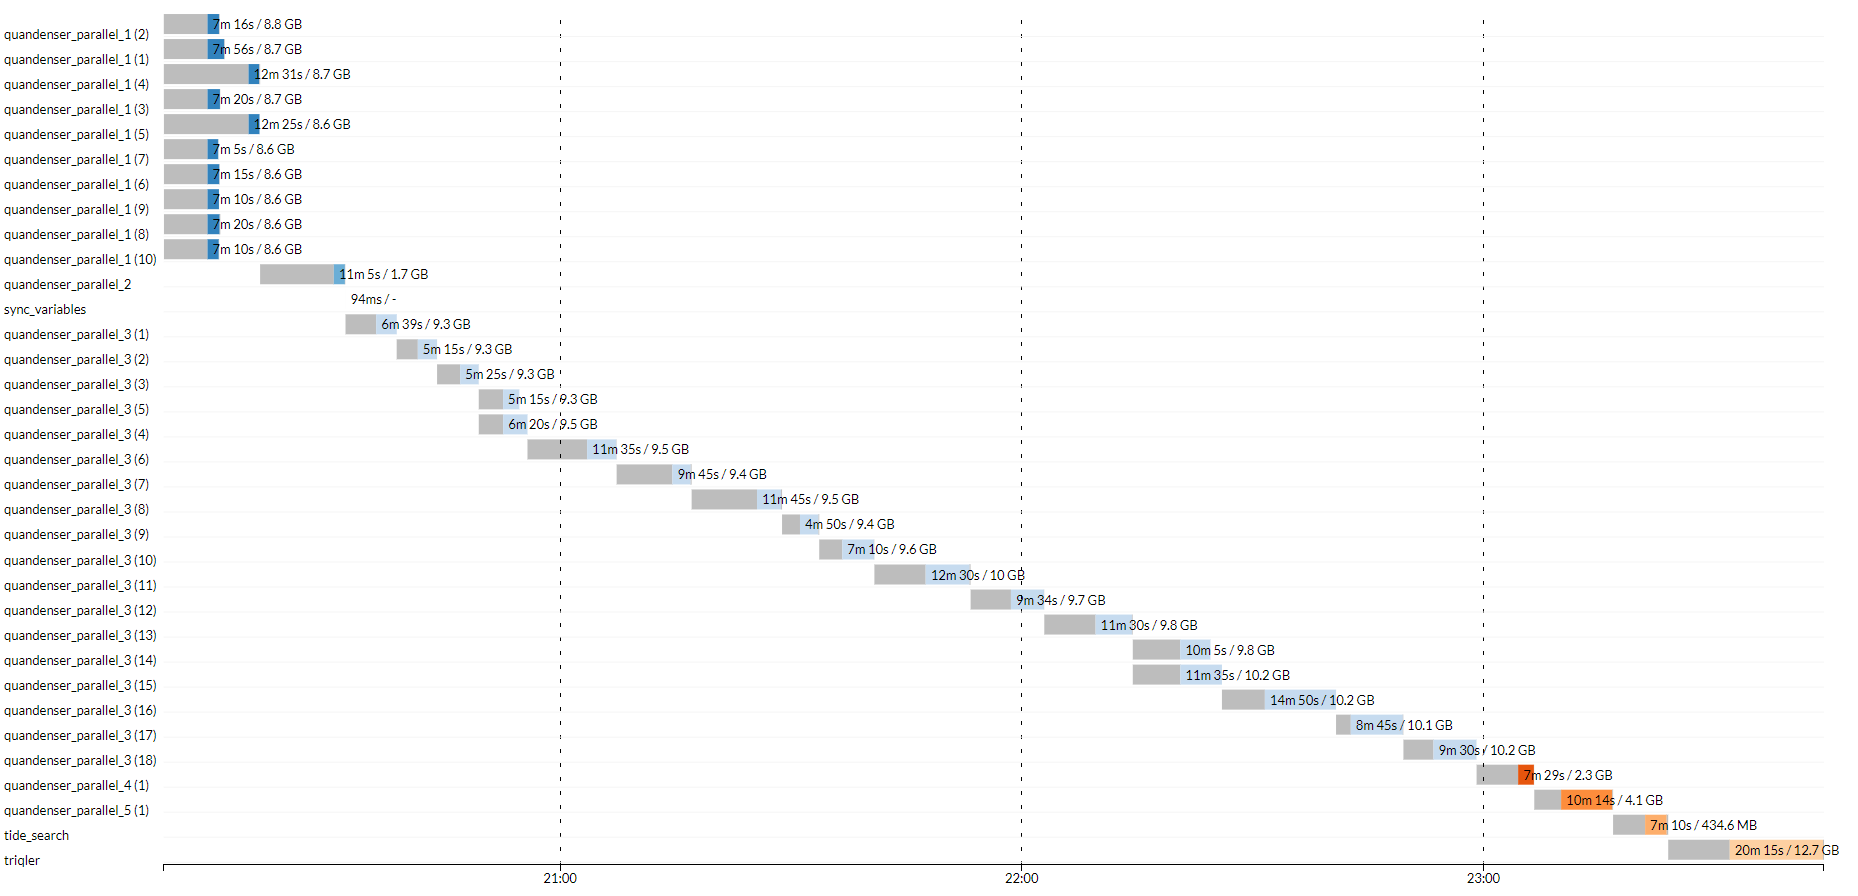
\includegraphics[width=\linewidth]{results/timeline-cluster.png}
  \caption{\textbf{Timeline of parallel processing of the cyanobacteria data set on UPPMAX.} The caption of figure \ref{fig:timeline-local} explains the processing names. The grey area of each bar represents SLURM queue time for each process. Unlimited amounts of processes was set, meaning no limit was set to the amount of parallelized processes possible}
  \label{fig:timeline-cluster}
\end{figure}

\subsection{Biological data}
The cyanobacteria experiment groups were divided in five groups; before sunrise (A), after sunrise (B), noon (C), before sunset (D) and after sunset (E) with two replicates each. From the cyanobacterial data set, each combination of experiment groups were compared to one another, i.e. all groups were compared to all other groups. For the ralstonia dataset, the same method applied where the experimental groups of 0.05, 0.10, 0.15, 0.20 and 0.25 growth-rate were compared to one another.

For the cyanobacteria dataset, a total of 24 proteins between the experimental groups were found to be differentially expressed, which consisted of 10 unique proteins (shown in table \ref{table:cyano-proteins}). For the ralstonia dataset, a total of 760 proteins between the experimental groups were found to be differentially expressed, which consisted of 267 unique proteins. Due to the large amount of unique proteins found in the ralstonia data set, the ralstonia proteins were not analyzed.

\begin{center}
\begin{table}[H]
\caption{\textbf{Differentially expressed proteins from the cyanobacteria data set}. Data about the function of the proteins were gathered from NCBI gene search \cite{ncbi-search}. PEP is the Posterior Error Probability of the protein, which is quite simply the probability that the observation is incorrect (in this case, if the protein found is what was in the mass analyzer) \cite{q-value}. Min q-value is the minimum q-value of the protein expression when comparing all experimental groups against one another.}
\begin{tabular}{ l l l l }
\toprule
Protein & Function & PEP & min q-value \\ \midrule
sll1214 & Magnesium-protoporphyrin IX monomethyl ester cyclase  & 6.305e-16 & 0.007298 \\ [0.5ex]
sll1184 & Heme oxygenase & 6.305e-16 & 0.00261 \\ [0.5ex]
slr2032 & Hypothetical protein YCF23 & 4.568e-13 & 0.03241 \\ [0.5ex]
sll1452 & Nitrate transport protein & 6.305e-16 & 0.01067 \\ [0.5ex]
ssl2501 & Hypothetical protein & 6.305e-16 & 0.002183 \\ [0.5ex]
ssr1480 & RNA-binding protein  & 6.305e-16 & 0.04116 \\ [0.5ex]
slr1739 & Photosystem II protein (PsbW) & 6.305e-16 & 0.04529 \\ [0.5ex]
ssr3383 & Phycobilisome LC linker polypeptide & 6.305e-16 & 0.006643 \\ [0.5ex]
slr0473 & Phytochrome Cph1 & 6.305e-16 & 0.02829 \\ [0.5ex]
slr0083 & ATP-dependent RNA helicase  & 6.305e-16 & 0.0164 \\ [0.5ex] \bottomrule
\end{tabular}
\centering
\label{table:cyano-proteins}
\end{table}
\end{center}

\begin{figure}[H]
  \begin{center}
  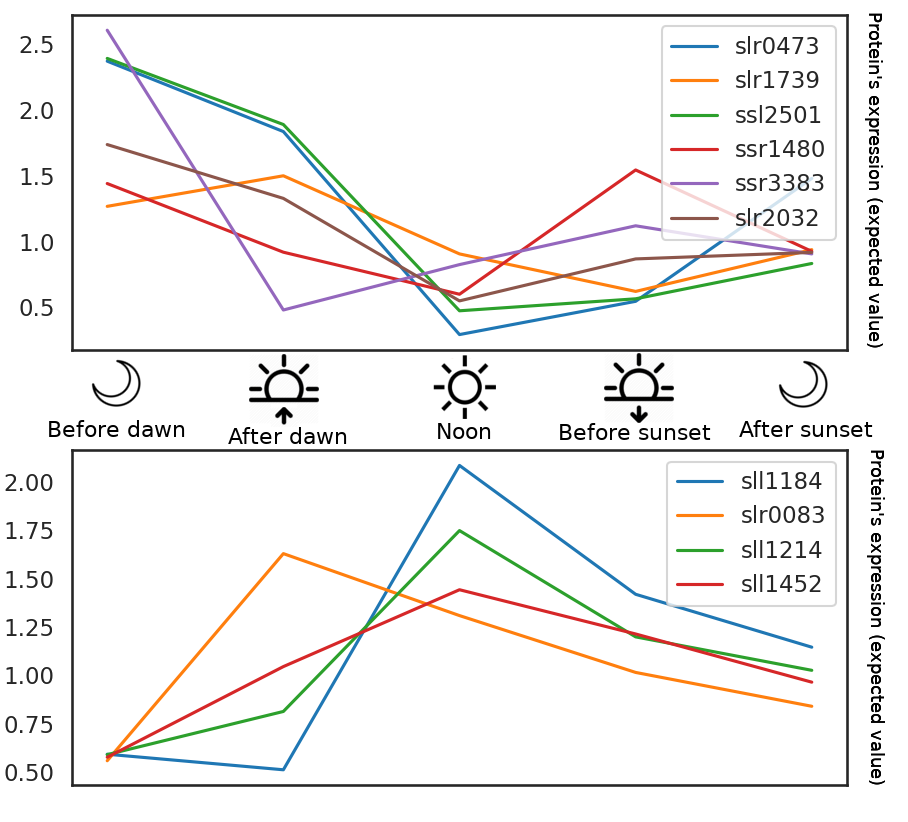
\includegraphics[width=\linewidth]{results/combined_edited.png}
  \caption{\textbf{Comparing protein expression of differentially expressed proteins.} The expected value of relative protein expression of the same protein, comparing the experimental groups from table \ref{table:cyano-proteins}. The experimental groups were cyanobacteria grown in conditions simulating; before sunrise, after sunrise, noon, before sundown and after sundown. The proteins in the plot were found to be differentially expressed and the "bands" of the lines are 95\% confidence interval around the mean. The proteins are divided into two plots; the top plot is proteins with a lower expression in the noon compared to before sunrise, while the plot at the bottom is proteins which has a higher expression during noon when comparing to before sunrise.}
  \label{fig:expression}
  \end{center}
\end{figure}

\section{Discussion}

\section{Conclusion}

Quandenser-pipeline is a mass spectrometry pipeline which is designed to be easy to use and as a wrapper for Quandenser and Triqler. The performance of the pipeline is better than MaxQuant on both data sets, but has a similar performance compared to the custom OpenMS pipeline, while the parallelization of Quandenser shows only a slight performance increase on smaller data sets compared to running the Quandenser in a non-parallel mode.

The biological data of differentially expressed proteins show us the how the proteome of cyanobacteria behaves during different times of the day, where the bacteria changes it's internal proteome to gather light from higher wavelengths before and after noon while changing it's energy metabolism to acclimate for the changes, which were confirmed in previous studies.

In conclusion; The pipeline allows an easy way of analyzing MS files with Quandenser, without requiring the user to convert vendor files to general MS files beforehand, while being accessible to run on HPC clusters with minimal dependencies. The processing time of the pipeline is also considerable faster than MaxQuant, a popular mass spectrometry analyzing software, and accessible on Linux computers without the need of other frameworks.

\section{Future work}

The pipeline has gotten some recognition over the course of its creating and has already been tested by researchers at SciLifeLab, Germany and Australia at the moment of writing. There are several improvements and future work that would be beneficial for the project.

\subsection{Further improvments of Quandenser parallelization}
The parallelization of the modified Quandenser could be improved in several fronts. The overhead calculations for the modified version of Quandenser when running in parallel slows down the processing time, which increases the total amount of core minutes required to complete the process, even though the real time processing is reduced. Some efforts has already been made to improve the overhead calculations by saving and loading parameters to temporary files, but the method of loading and saving data is rather slow and results in stability issues. However, the results only gives an insignificant speed boost for the processing and could be further improved.

As explained in the method section \ref{ssec:quandenser-method}, the parallelization of the minimum spanning tree cannot be "fully" parallelized (i.e. run all the calculations at the same time) and is unstable for large cohorts, due to the efforts to reduce overhead calculations mentioned above. Possible improvements in the modified version of Quandenser to rearrange the structure of minimum spanning tree to maximize the amount of possible parallel computations could improve the calculation times for larger cohorts of samples.

In summary, by further improving how the modified Quandenser loads and saves data from previous runs and rearranging the minimum depth tree would yield significant improvements of parallel computation times and stability of the parallel Quandenser option of the pipeline, which in turn would result in an even faster processing speed-

\subsection{Analyzing boxcar spectra}
A novel method of mass spectrometry data acquisition has been developed by researches at Matthias Mann Lab in Munich, which increases the resolution of MS1 spectra by making one low resolution MS1 scan and then multiple, smaller high resolution MS1 scans in chunks \cite{boxcar}. A custom python script was created and integrated into the latest version of Quandenser-pipeline (v0.071) to be able to utilize the new type of data from the data acquisition. By enabling the option in the pipeline, all mzML files (including any non-mzML mass spectrometry files after conversion) will be analyzed for Boxcar spectra and merged if found. The script merges MS1 and Boxcar in mzML files for processing in Quandenser, then restructures and outputs a new mzML file with combined MS1 spectra. The resulting file has an increased resolution compared to regular MS1 scans.

A data set with boxcar data could possibly be analyzed with the new pipeline to test how the increased resolution of MS1 spectra would yield for results. One such data set exists with patients where blood samples before and after gastric bypass surgery were taken, which were then run through the new Boxcar acquisition method \cite{boxcar-data}.

\section{Acknowledgements}

I would like to thank the following persons for their support of the project:

Lukas Käll: The supervisor of the project, for helping me set up the programs used in the pipeline, providing a computer to work on and guidance during the project.

Michael Jahn: The secondary supervisor of the project, for helping me set up the OpenMS pipeline and for providing the data sets analyzed in the thesis.

Peter Savolainen: The examiner of the project, for taking me in as a thesis student and grading the project.

Matthew The: The author of several reports cited in the thesis, for creating the software Quandenser + Triqler alongside Lukas Käll.

Patrick Troung, Marcus Ekvall and Gus Jeuken: PhD students and research engineers working at Käll lab, for helping me with various programming issues and for testing the pipeline.

\newpage
\printbibliography[heading=bibnumbered]
\newpage
\section{Appendix}

Quandenser-pipeline on github: \url{https://github.com/statisticalbiotechnology/quandenser-pipeline}
Modified Quandenser on github: \url{https://github.com/statisticalbiotechnology/quandenser/tree/quandenser-pipeline}
OpenMS pipeline by Michael Jahn: \url{https://github.com/m-jahn/openMS-workflows}


\begin{center}
\begin{longtable}{ l l l l }
\caption{\textbf{Differentially expressed proteins from the ralstonia data set}. Data about the function of the proteins were gathered from a custom fasta file, used for the processing of the data}\\
\toprule
Protein & Function & PEP & min q-value \\\midrule
HEMN\_CUPNH & Oxygen-independent coproporphyrinogen III oxidase& 1.072e-14 & 0.01182 \\ [0.5ex]
FDHD\_CUPNH & Sulfur carrier protein FdhD& 6.305e-16 & 0.0008676 \\ [0.5ex]
F16A2\_CUPNH & Fructose-1,6-bisphosphatase class 1 2& 6.305e-16 & 0.02997 \\ [0.5ex]
TKTC\_CUPNH & Transketolase, chromosomal& 6.305e-16 & 0.0002889 \\ [0.5ex]
TKTP\_CUPNH & Transketolase, plasmid& 6.305e-16 & 0.03531 \\ [0.5ex]
HOXF\_CUPNH & NAD-reducing hydrogenase HoxS subunit alpha& 6.305e-16 & 0.01562 \\ [0.5ex]
HMP\_CUPNH & Flavohemoprotein& 6.305e-16 & 1.243e-05 \\ [0.5ex]
GPHC\_CUPNH & Phosphoglycolate phosphatase, chromosomal& 6.305e-16 & 0.004352 \\ [0.5ex]
GPHP\_CUPNH & Phosphoglycolate phosphatase, plasmid& 6.305e-16 & 0.002978 \\ [0.5ex]
PGKC\_CUPNH & Phosphoglycerate kinase, chromosomal& 6.305e-16 & 0.01915 \\ [0.5ex]
Q0JY25\_CUPNH & Phosphogluconate dehydratase& 3.16e-08 & 0.04928 \\ [0.5ex]
Q0JY28\_CUPNH & Glucokinase& 6.305e-16 & 0.006335 \\ [0.5ex]
Q0JY90\_CUPNH & ABC-type transporter, periplasmic component& 6.305e-16 & 0.01285 \\ [0.5ex]
Q0JY94\_CUPNH & Intracellular protease/amidase& 6.305e-16 & 1.96e-05 \\ [0.5ex]
Q0JY96\_CUPNH & 3-Oxoacyl-[acyl-carrier protein] reductase& 6.305e-16 & 0.04771 \\ [0.5ex]
Q0JYF3\_CUPNH & Probable extra-cytoplasmic solute receptor& 6.305e-16 & 0.01973 \\ [0.5ex]
Q0JYF8\_CUPNH & Uncharacterized protein& 6.305e-16 & 0.0002473 \\ [0.5ex]
Q0JYF9\_CUPNH & Uncharacterized protein& 6.305e-16 & 0.000112 \\ [0.5ex]
Q0JYG0\_CUPNH & Uncharacterized protein& 6.305e-16 & 0.0003117 \\ [0.5ex]
Q0JYG9\_CUPNH & Periplasmic solute binding protein& 6.305e-16 & 6.948e-06 \\ [0.5ex]
Q0JYI9\_CUPNH & Periplasmic alpha-carbonic anhydrase& 6.305e-16 & 0.0007225 \\ [0.5ex]
Q0JYJ5\_CUPNH & Acetyltransferase& 6.305e-16 & 0.02146 \\ [0.5ex]
Q0JYN2\_CUPNH & Flagellin& 6.305e-16 & 0.02032 \\ [0.5ex]
Q0JYT4\_CUPNH & Probable extra-cytoplasmic solute receptor& 6.305e-16 & 0.03699 \\ [0.5ex]
Q0JYZ2\_CUPNH & Uncharacterized protein& 7.525e-14 & 0.003195 \\ [0.5ex]
Q0JZ03\_CUPNH & Peroxiredoxin& 6.305e-16 & 0.003645 \\ [0.5ex]
Q0JZ56\_CUPNH & Response regulator of copper response y& 6.305e-16 & 0.02144 \\ [0.5ex]
Q0JZ57\_CUPNH & Copper resistance protein A, multi-copper oxidase& 6.305e-16 & 3.416e-05 \\ [0.5ex]
Q0JZ59\_CUPNH & Copper resistance protein C& 6.305e-16 & 0.01852 \\ [0.5ex]
Q0JZA6\_CUPNH & Uncharacterized protein& 6.305e-16 & 0.003084 \\ [0.5ex]
Q0JZL7\_CUPNH & Cold shock protein, DNA-binding& 6.305e-16 & 0.01379 \\ [0.5ex]
Q0JZM1\_CUPNH & Phasin& 6.305e-16 & 5.764e-05 \\ [0.5ex]
Q0JZU7\_CUPNH & Glutamate dehydrogenase& 5.566e-12 & 0.024 \\ [0.5ex]
Q0JZU9\_CUPNH & Putative non-heme chloroperoxidase& 2.578e-14 & 0.0005583 \\ [0.5ex]
Q0JZV8\_CUPNH & Uncharacterized protein& 6.305e-16 & 4.886e-05 \\ [0.5ex]
Q0JZW1\_CUPNH & Isocitrate dehydrogenase [NADP]& 6.305e-16 & 0.04057 \\ [0.5ex]
Q0K0J0\_CUPNH & Zinc-type alcohol dehydrogenase-like protein& 1.755e-12 & 0.01944 \\ [0.5ex]
Q0K0J7\_CUPNH & Putative aminotransferase& 6.305e-16 & 0.01058 \\ [0.5ex]
Q0K0K1\_CUPNH & Pyoverdine biosynthesis regulatory protein& 6.305e-16 & 0.0001744 \\ [0.5ex]
Q0K0K2\_CUPNH & Non-ribosomal peptide synthetase& 6.305e-16 & 0.002946 \\ [0.5ex]
Q0K0K8\_CUPNH & Siderophore biosynthesis related protein& 6.305e-16 & 0.006121 \\ [0.5ex]
Q0K0K9\_CUPNH & Lysine/ornithine N-monooxygenase& 0.02093 & 0.02442 \\ [0.5ex]
Q0K0P4\_CUPNH & Uncharacterized protein& 6.305e-16 & 0.0002406 \\ [0.5ex]
Q0K0T9\_CUPNH & ABC-type transporter, periplasmic component& 6.305e-16 & 0.005414 \\ [0.5ex]
Q0K0U4\_CUPNH & Uracil phosphoribosyltransferase& 6.37e-06 & 0.003867 \\ [0.5ex]
Q0K0U9\_CUPNH & Zn-dependent hydrolase & 6.305e-16 & 0.007052 \\ [0.5ex]
Q0K0V5\_CUPNH & Uncharacterized protein& 6.305e-16 & 0.000398 \\ [0.5ex]
METE\_CUPNH & 5-methyltetrahydropteroyltriglutamate& 6.305e-16 & 0.0001278 \\ [0.5ex]
Q0K0W3\_CUPNH & Beta-lactamase class C& 2.008e-09 & 0.003304 \\ [0.5ex]
Q0K128\_CUPNH & Probable extra-cytoplasmic solute receptor& 6.164e-14 & 0.03407 \\ [0.5ex]
Q0K184\_CUPNH & Formate dehydrogenase alpha subunit& 6.305e-16 & 0.03316 \\ [0.5ex]
Q0K188\_CUPNH & Probable extra-cytoplasmic solute receptor& 6.305e-16 & 0.01765 \\ [0.5ex]
Q0K1C9\_CUPNH & Predicted nucleoside-diphosphate-sugar epimerase& 6.305e-16 & 0.003393 \\ [0.5ex]
Q0K1D0\_CUPNH & Alkyl hydroperoxide reductase AhpD& 6.305e-16 & 0.0001293 \\ [0.5ex]
Q0K1F2\_CUPNH & Formate dehydrogenase, alpha chain& 6.305e-16 & 0.04192 \\ [0.5ex]
Q0K1F4\_CUPNH & Uncharacterized protein& 5.769e-15 & 0.04284 \\ [0.5ex]
Q0K1I7\_CUPNH & Putative peptidase, C56 family& 6.305e-16 & 0.001184 \\ [0.5ex]
Q0K1Q4\_CUPNH & Probable extra-cytoplasmic solute receptor& 6.305e-16 & 0.006607 \\ [0.5ex]
Q0K1S5\_CUPNH & Uncharacterized protein& 6.305e-16 & 0.00592 \\ [0.5ex]
Q0K1X1\_CUPNH & 2-Keto-3-deoxy-6-phosphogluconate aldolase& 6.305e-16 & 0.03162 \\ [0.5ex]
Q0K1X3\_CUPNH & Amino acid aldolase or racemase& 6.305e-16 & 0.01705 \\ [0.5ex]
Q0K240\_CUPNH & Lactoylglutathione lyase& 1.258e-13 & 0.002179 \\ [0.5ex]
Q0K241\_CUPNH & NADH:flavin oxidoreductase / NADH oxidase family& 6.305e-16 & 0.004832 \\ [0.5ex]
Q0K278\_CUPNH & Putative peptidase, M20A subfamily& 6.305e-16 & 0.0001523 \\ [0.5ex]
Q0K2A2\_CUPNH & Tyrosine aminotransferase& 6.305e-16 & 0.00462 \\ [0.5ex]
Q0K2A7\_CUPNH & Phospho-2-dehydro-3-deoxyheptonate aldolase& 6.305e-16 & 0.02087 \\ [0.5ex]
Q0K308\_CUPNH & D-3-Phosphoglycerate dehydrogenase& 6.305e-16 & 0.0291 \\ [0.5ex]
Q0K334\_CUPNH & Ankyrin repeat protein containing four repeats& 6.305e-16 & 0.00653 \\ [0.5ex]
Q0K338\_CUPNH & TRAP-type transporter, periplasmic component& 6.305e-16 & 6.008e-07 \\ [0.5ex]
Q0K368\_CUPNH & Acetyl-CoA acetyltransferase& 6.305e-16 & 0.03121 \\ [0.5ex]
Q0K371\_CUPNH & Enoyl-CoA hydratase& 6.305e-16 & 0.0009203 \\ [0.5ex]
Q0K3B4\_CUPNH & Short-chain alcohol dehydrogenase& 6.305e-16 & 4.834e-05 \\ [0.5ex]
Q0K3C7\_CUPNH & Serine protein kinase& 6.305e-16 & 0.0113 \\ [0.5ex]
Q0K3J1\_CUPNH & Uncharacterized protein& 6.305e-16 & 0.01153 \\ [0.5ex]
Q0K3N5\_CUPNH & Uncharacterized protein& 3.279e-12 & 0.04238 \\ [0.5ex]
Q0K3Q3\_CUPNH & Ubiquinone/menaquinone biosynthesis methyltransferase& 6.305e-16 & 0.04472 \\ [0.5ex]
Q0K3Y3\_CUPNH & Cysteine desulfurase IscS& 6.305e-16 & 0.01852 \\ [0.5ex]
Q0K4E2\_CUPNH & NADPH:quinone reductase & 6.305e-16 & 0.008572 \\ [0.5ex]
Q0K4E3\_CUPNH & Probable extra-cytoplasmic solute receptor& 5.426e-09 & 0.0462 \\ [0.5ex]
Q0K4J3\_CUPNH & Dihydroxy-acid dehydratase& 6.305e-16 & 0.01553 \\ [0.5ex]
Q0K513\_CUPNH & Ferredoxin& 5.803e-07 & 0.03489 \\ [0.5ex]
Q0K515\_CUPNH & Fumarate hydratase class II& 6.305e-16 & 0.04875 \\ [0.5ex]
Q0K552\_CUPNH & Probable extra-cytoplasmic solute receptor& 6.305e-16 & 0.03725 \\ [0.5ex]
Q0K557\_CUPNH & ABC-type transporter, periplasmic component& 6.305e-16 & 0.009592 \\ [0.5ex]
Q0K5E1\_CUPNH & Dihydrolipoamide dehydrogenase& 6.305e-16 & 0.02002 \\ [0.5ex]
Q0K5E7\_CUPNH & Probable extra-cytoplasmic solute receptor & 6.305e-16 & 0.02435 \\ [0.5ex]
Q0K5G4\_CUPNH & Putative peptidoglycan binding domain& 6.305e-16 & 0.005667 \\ [0.5ex]
Q0K5J5\_CUPNH & Copper chaperone, heavy metal ion binding& 6.305e-16 & 0.01535 \\ [0.5ex]
Q0K5K4\_CUPNH & ABC-type transporter, periplasmic component& 6.305e-16 & 0.01766 \\ [0.5ex]
Q0K5K9\_CUPNH & ABC-type transporter, periplasmic component& 6.305e-16 & 0.002447 \\ [0.5ex]
Q0K5N5\_CUPNH & Uncharacterized protein& 6.305e-16 & 8.121e-06 \\ [0.5ex]
Q0K5S1\_CUPNH & Short chain dehydrogenase& 6.305e-16 & 0.0292 \\ [0.5ex]
Q0K5S5\_CUPNH & Putative peptidase, M20A subfamily& 6.305e-16 & 0.006939 \\ [0.5ex]
Q0K5S8\_CUPNH & Arsenate reductase& 6.305e-16 & 0.01179 \\ [0.5ex]
RL4\_CUPNH & 50S ribosomal protein L4& 6.305e-16 & 0.04309 \\ [0.5ex]
RL2\_CUPNH & 50S ribosomal protein L2& 6.305e-16 & 0.04823 \\ [0.5ex]
RL16\_CUPNH & 50S ribosomal protein L16& 6.305e-16 & 0.01732 \\ [0.5ex]
RL24\_CUPNH & 50S ribosomal protein L24& 6.305e-16 & 0.01234 \\ [0.5ex]
Q0K663\_CUPNH & Type IV pilus assembly protein PilM& 6.305e-16 & 0.0002645 \\ [0.5ex]
Q0K667\_CUPNH & Pili assembly protein PilQ& 6.305e-16 & 0.0001532 \\ [0.5ex]
Q0K673\_CUPNH & Glutamate synthase [NADPH] small chain& 6.305e-16 & 0.001244 \\ [0.5ex]
Q0K6B3\_CUPNH & Response regulator & 6.305e-16 & 0.02058 \\ [0.5ex]
Q0K6F2\_CUPNH & Probable extra-cytoplasmic solute receptor& 6.305e-16 & 0.002093 \\ [0.5ex]
Q0K6G5\_CUPNH & S-adenosylhomocysteine nucleosidase& 6.305e-16 & 0.03184 \\ [0.5ex]
Q0K6H2\_CUPNH & Alcohol dehydrogenase& 6.305e-16 & 0.003757 \\ [0.5ex]
Q0K6I3\_CUPNH & Anthranilate synthase component 1& 6.305e-16 & 0.001129 \\ [0.5ex]
Q0K6I8\_CUPNH & Membrane-bound lytic murein transglycosylase& 6.305e-16 & 0.02836 \\ [0.5ex]
Q0K6J9\_CUPNH & ABC-type transporter, periplasmic component & 6.305e-16 & 7.137e-05 \\ [0.5ex]
Q0K6K4\_CUPNH & ABC-type transporter, periplasmic component& 6.305e-16 & 0.001537 \\ [0.5ex]
Q0K6L2\_CUPNH & Probable extra-cytoplasmic solute receptor& 6.305e-16 & 0.00715 \\ [0.5ex]
Q0K6M0\_CUPNH & UDP-N-acetylmuramoyl-tripeptide & 6.305e-16 & 0.01018 \\ [0.5ex]
Q0K6N0\_CUPNH & Peroxiredoxin& 6.305e-16 & 0.01675 \\ [0.5ex]
SECA\_CUPNH & Protein translocase subunit SecA& 6.305e-16 & 0.005118 \\ [0.5ex]
Q0K6N5\_CUPNH & Predicted ATPase, AAA+ superfamily& 6.305e-16 & 0.02365 \\ [0.5ex]
Q0K6Q5\_CUPNH & Signal recognition particle protein& 6.305e-16 & 0.02964 \\ [0.5ex]
Q0K6V5\_CUPNH & Probable extra-cytoplasmic solute receptor& 8.473e-11 & 0.00423 \\ [0.5ex]
Q0K6W0\_CUPNH & Aldehyde reductase, related to diketogulonate reductase& 6.305e-16 & 0.006651 \\ [0.5ex]
Q0K6X4\_CUPNH & Biotin carboxylase& 6.305e-16 & 0.03079 \\ [0.5ex]
Q0K6Y2\_CUPNH & Predicted short chain dehydrogenase& 6.305e-16 & 3.804e-05 \\ [0.5ex]
Q0K704\_CUPNH & Outer membrane protein assembly factor BamE& 6.305e-16 & 0.02762 \\ [0.5ex]
Q0K707\_CUPNH & Leucine--tRNA ligase& 6.305e-16 & 0.009664 \\ [0.5ex]
Q0K742\_CUPNH & Type IV pilus twitching motility protein PilT& 6.305e-16 & 0.004472 \\ [0.5ex]
Q0K743\_CUPNH & Type IV pilus twitching motility protein PilU& 6.305e-16 & 0.04584 \\ [0.5ex]
Q0K744\_CUPNH & Glutathione peroxidase& 6.305e-16 & 0.007141 \\ [0.5ex]
Q0K753\_CUPNH & Acetyltransferase& 6.305e-16 & 0.0265 \\ [0.5ex]
Q0K773\_CUPNH & Hydantoin racemase& 2.289e-09 & 0.01262 \\ [0.5ex]
Q0K791\_CUPNH & Uncharacterized protein& 1.424e-09 & 0.0001892 \\ [0.5ex]
Q0K7A8\_CUPNH & Quinolinate synthase A& 6.305e-16 & 0.02198 \\ [0.5ex]
Q0K7B5\_CUPNH & 4-hydroxy-3-methylbut-2-enyl diphosphate reductase& 4.783e-13 & 0.04521 \\ [0.5ex]
Q0K7B6\_CUPNH & ABC-type transporter, periplasmic component & 6.305e-16 & 0.04318 \\ [0.5ex]
Q0K7C0\_CUPNH & ABC-type transporter, ATPase component& 6.305e-16 & 0.02254 \\ [0.5ex]
Q0K7C4\_CUPNH & ABC-type transporter, periplasmic component& 5.817e-14 & 0.01408 \\ [0.5ex]
Q0K7E6\_CUPNH & Sulfite reductase, beta subunit& 6.305e-16 & 0.01999 \\ [0.5ex]
Q0K7E9\_CUPNH & Sulfate adenylyltransferase subunit 2& 6.305e-16 & 0.004106 \\ [0.5ex]
Q0K7F0\_CUPNH & Sulfate adenylyltransferase subunit 1& 6.305e-16 & 0.01478 \\ [0.5ex]
Q0K7G7\_CUPNH & Acyl-CoA synthetase& 6.305e-16 & 0.0006265 \\ [0.5ex]
Q0K7H0\_CUPNH & Uncharacterized protein& 6.305e-16 & 0.04513 \\ [0.5ex]
PYRB\_CUPNH & Aspartate carbamoyltransferase& 6.305e-16 & 0.02967 \\ [0.5ex]
Q0K7N3\_CUPNH & Dihydroorotase& 6.305e-16 & 0.00354 \\ [0.5ex]
Q0K7P5\_CUPNH & GDP-mannose 4,6-dehydratase& 6.305e-16 & 0.0005956 \\ [0.5ex]
Q0K7Q2\_CUPNH & Putative glucose-1-phosphate cytidylyltransferase& 6.305e-16 & 0.0204 \\ [0.5ex]
Q0K7Y9\_CUPNH & Cyclopropane fatty acid synthase& 6.305e-16 & 0.0006946 \\ [0.5ex]
Q0K7Z5\_CUPNH & Hemerythrin& 2.356e-12 & 0.04331 \\ [0.5ex]
KATG\_CUPNH & Catalase-peroxidase& 6.305e-16 & 0.0004172 \\ [0.5ex]
GCH4\_CUPNH & GTP cyclohydrolase FolE2& 6.305e-16 & 0.01072 \\ [0.5ex]
Q0K875\_CUPNH & ATP-dependent helicase & 6.305e-16 & 0.007933 \\ [0.5ex]
Q0K878\_CUPNH & Pirin-related protein& 1.021e-09 & 0.004154 \\ [0.5ex]
Q0K893\_CUPNH & ATP-dependent RNA helicase& 6.305e-16 & 0.000363 \\ [0.5ex]
Q0K8C9\_CUPNH & Transcriptional regulator, MocR family& 6.305e-16 & 0.0336 \\ [0.5ex]
HTPG\_CUPNH & Chaperone protein HtpG& 6.305e-16 & 0.003416 \\ [0.5ex]
Q0K8G2\_CUPNH & Citrate synthase& 6.305e-16 & 0.03493 \\ [0.5ex]
Q0K8G8\_CUPNH & 3-isopropylmalate dehydratase large subunit& 6.305e-16 & 0.01437 \\ [0.5ex]
Q0K8H1\_CUPNH & Aspartate-semialdehyde dehydrogenase& 6.305e-16 & 0.01293 \\ [0.5ex]
Q0K8I3\_CUPNH & O-succinylhomoserine sulfhydrylase& 6.305e-16 & 0.02065 \\ [0.5ex]
Q0K8I8\_CUPNH & 30S ribosomal protein S21& 6.305e-16 & 0.02753 \\ [0.5ex]
FENR2\_CUPNH & Ferredoxin--NADP reductase 2& 6.305e-16 & 0.02918 \\ [0.5ex]
Q0K8Q6\_CUPNH & Fumarate hydratase class I& 6.305e-16 & 0.03539 \\ [0.5ex]
Q0K8R9\_CUPNH & Uncharacterized protein& 7.91e-13 & 0.002453 \\ [0.5ex]
Q0K8S1\_CUPNH & Uncharacterized protein& 1.668e-10 & 0.01603 \\ [0.5ex]
Q0K8T5\_CUPNH & ABC-type sugar transporter, periplasmic component& 6.305e-16 & 0.0007247 \\ [0.5ex]
Q0K8X8\_CUPNH & Carbamoyl-phosphate synthase small chain& 6.305e-16 & 0.01583 \\ [0.5ex]
GLMM\_CUPNH & Phosphoglucosamine mutase& 6.305e-16 & 0.002126 \\ [0.5ex]
Q0K8Y8\_CUPNH & Phosphate-binding protein PstS& 6.305e-16 & 0.03277 \\ [0.5ex]
RLMD\_CUPNH & 23S rRNA& 6.305e-16 & 0.003103 \\ [0.5ex]
SYH\_CUPNH & Histidine--tRNA ligase& 6.305e-16 & 0.02549 \\ [0.5ex]
Q0K9D1\_CUPNH & GTP-binding elongation factor family protein& 6.305e-16 & 0.004461 \\ [0.5ex]
Q0K9D4\_CUPNH & Probable enoyl-CoA hydratase& 6.305e-16 & 0.00906 \\ [0.5ex]
Q0K9D5\_CUPNH & Acyl carrier protein phosphodiesterase& 6.305e-16 & 0.002008 \\ [0.5ex]
Q0K9F7\_CUPNH & Aspartate/tyrosine/aromatic aminotransferase& 6.305e-16 & 0.01104 \\ [0.5ex]
Q0K9F9\_CUPNH & Threonine synthase& 6.305e-16 & 0.01324 \\ [0.5ex]
Q0K9K4\_CUPNH & Universal stress protein, UspA family& 6.305e-16 & 0.01423 \\ [0.5ex]
Q0K9K8\_CUPNH & SAM-dependent methyltransferase& 6.305e-16 & 0.00255 \\ [0.5ex]
Q0K9K9\_CUPNH & Dienelactone hydrolase or related enzyme& 6.305e-16 & 0.0008204 \\ [0.5ex]
Q0K9Q2\_CUPNH & Phasin& 6.305e-16 & 0.004308 \\ [0.5ex]
Q0K9R3\_CUPNH & Universal stress protein, UspA family& 6.305e-16 & 5.635e-06 \\ [0.5ex]
Q0K9R7\_CUPNH & Uncharacterized protein& 3.898e-11 & 0.0001386 \\ [0.5ex]
Q0KA24\_CUPNH & Outer membrane protein assembly factor BamA& 6.305e-16 & 0.01888 \\ [0.5ex]
FABZ\_CUPNH & 3-hydroxyacyl-[acyl-carrier-protein] dehydratase FabZ& 6.305e-16 & 0.005558 \\ [0.5ex]
Q0KA29\_CUPNH & Lipid-A-disaccharide synthase& 6.305e-16 & 0.02198 \\ [0.5ex]
Q0KA31\_CUPNH & 23S rRNA methyltransferase& 6.305e-16 & 0.04614 \\ [0.5ex]
Q0KA33\_CUPNH & Phosphoenolpyruvate synthase& 6.305e-16 & 0.04098 \\ [0.5ex]
Q0KA35\_CUPNH & Membrane protease subunits, stomatin & 6.305e-16 & 0.02724 \\ [0.5ex]
Q0KAE4\_CUPNH & Uncharacterized protein conserved in bacteria& 6.305e-16 & 0.02303 \\ [0.5ex]
Q0KAE9\_CUPNH & ABC-type transporter, duplicated ATPase domains & 6.305e-16 & 0.01099 \\ [0.5ex]
Q0KAG0\_CUPNH & Glutaminase-asparaginase& 6.305e-16 & 5.567e-05 \\ [0.5ex]
Q0KAG5\_CUPNH & 2-methylisocitrate lyase& 6.305e-16 & 0.02577 \\ [0.5ex]
Q0KAI7\_CUPNH & Probable extra-cytoplasmic solute receptor& 6.305e-16 & 0.003685 \\ [0.5ex]
Q0KB05\_CUPNH & Predicted oxidoreductas& 2.708e-10 & 0.001436 \\ [0.5ex]
Q0KB40\_CUPNH & 3-Demethylubiquinone-9 3-methyltransferase& 6.305e-16 & 0.0002093 \\ [0.5ex]
Q0KB41\_CUPNH & Glutathione S-transferase& 6.305e-16 & 0.001076 \\ [0.5ex]
Q0KB43\_CUPNH & Probable extra-cytoplasmic solute receptor& 6.305e-16 & 0.04167 \\ [0.5ex]
Q0KB97\_CUPNH & Hypothetical membrane spanning protein& 6.305e-16 & 0.008809 \\ [0.5ex]
Q0KBD4\_CUPNH & Probable extra-cytoplasmic solute receptor& 6.305e-16 & 0.0283 \\ [0.5ex]
Q0KBD7\_CUPNH & Predicted phosphatase homolog & 6.305e-16 & 0.0003859 \\ [0.5ex]
Q0KBF3\_CUPNH & Uncharacterized protein& 6.305e-16 & 0.01796 \\ [0.5ex]
Q0KBF8\_CUPNH & Short chain dehydrogenase& 6.305e-16 & 0.017 \\ [0.5ex]
Q0KBG5\_CUPNH & ABC-type transporter, ATPase component & 1.765e-10 & 0.007887 \\ [0.5ex]
Q0KBG9\_CUPNH & ABC-type transporter, periplasmic component & 6.305e-16 & 1.929e-05 \\ [0.5ex]
CLPX\_CUPNH & ATP-dependent Clp protease ATP-binding & 6.305e-16 & 0.01797 \\ [0.5ex]
Q0KBQ7\_CUPNH & Transcriptional accessory protein& 6.305e-16 & 0.001863 \\ [0.5ex]
Q0KBR2\_CUPNH & Molecular chaperone, HSP20 family& 6.305e-16 & 0.024 \\ [0.5ex]
SYT\_CUPNH & Threonine--tRNA ligase& 6.305e-16 & 0.01446 \\ [0.5ex]
Q0KCF0\_CUPNH & Uncharacterized conserved protein& 6.305e-16 & 0.02239 \\ [0.5ex]
Q0KCF1\_CUPNH & Gluconokinase& 6.305e-16 & 0.02116 \\ [0.5ex]
SYK\_CUPNH & Lysine--tRNA ligase& 6.305e-16 & 0.001926 \\ [0.5ex]
Q0KCH9\_CUPNH & Aminotransferase& 6.305e-16 & 0.007923 \\ [0.5ex]
Q0KCI8\_CUPNH & Putative NADH dehydrogenase/NAD & 6.305e-16 & 0.000477 \\ [0.5ex]
Q0KCJ8\_CUPNH & NAD kinase& 6.305e-16 & 0.008097 \\ [0.5ex]
Q0KCK8\_CUPNH & Phospho-2-dehydro-3-deoxyheptonate aldolase& 6.305e-16 & 0.01292 \\ [0.5ex]
Q0KCM0\_CUPNH & Probable extra-cytoplasmic solute receptor& 6.305e-16 & 0.001469 \\ [0.5ex]
Q0KCM6\_CUPNH & Aspartate/tyrosine/aromatic aminotransferase& 6.305e-16 & 0.03868 \\ [0.5ex]
Q0KCP0\_CUPNH & Glutathione S-transferase& 6.305e-16 & 0.04377 \\ [0.5ex]
NUOC\_CUPNH & NADH-quinone oxidoreductase subunit C& 6.305e-16 & 0.02794 \\ [0.5ex]
NUOB\_CUPNH & NADH-quinone oxidoreductase subunit B& 6.305e-16 & 0.04207 \\ [0.5ex]
Q0KCT9\_CUPNH & Uncharacterized protein containing LysM domain& 6.305e-16 & 0.0005918 \\ [0.5ex]
ILVC\_CUPNH & Ketol-acid reductoisomerase& 6.305e-16 & 0.03038 \\ [0.5ex]
Q0KCU4\_CUPNH & Acetolactate synthase& 6.305e-16 & 0.04424 \\ [0.5ex]
Q0KCW0\_CUPNH & ABC-type transporter & 6.305e-16 & 0.02614 \\ [0.5ex]
Q0KCY5\_CUPNH & Membrane protein& 9.977e-11 & 0.007849 \\ [0.5ex]
Q0KD42\_CUPNH & Zinc-binding dehydrogenase& 6.305e-16 & 0.006841 \\ [0.5ex]
Y899\_CUPNH & UPF0176 protein H16\_A0899& 6.305e-16 & 0.005971 \\ [0.5ex]
RL19\_CUPNH & 50S ribosomal protein L19& 6.305e-16 & 0.01856 \\ [0.5ex]
HLDD\_CUPNH & ADP-L-glycero-D-manno-heptose-6-epimerase& 6.305e-16 & 0.0436 \\ [0.5ex]
Q0KDH2\_CUPNH & UDP-glucose 6-dehydrogenase& 6.305e-16 & 0.002759 \\ [0.5ex]
Q0KDJ9\_CUPNH & Cyanophycin synthetase& 6.305e-16 & 0.03915 \\ [0.5ex]
Q0KDK3\_CUPNH & ABC-type transporter, periplasmic component & 6.305e-16 & 0.02298 \\ [0.5ex]
ADH\_CUPNH & Alcohol dehydrogenase& 6.305e-16 & 2.716e-05 \\ [0.5ex]
Q0KDR5\_CUPNH & Uncharacterized protein& 1.729e-08 & 0.02265 \\ [0.5ex]
Q0KDS2\_CUPNH & Aerobic-type carbon monoxide dehydrogenase homolog & 6.305e-16 & 0.005064 \\ [0.5ex]
Q0KDY2\_CUPNH & NAD-dependent formate dehydrogenase beta subunit& 6.305e-16 & 0.009924 \\ [0.5ex]
Q0KE04\_CUPNH & YcaC related amidohydrolase& 3.823e-12 & 0.001086 \\ [0.5ex]
RECA\_CUPNH & Protein RecA& 6.305e-16 & 0.01886 \\ [0.5ex]
Q0KE88\_CUPNH & Universal stress protein, UspA family& 6.305e-16 & 0.04921 \\ [0.5ex]
Q0KEC5\_CUPNH & Uncharacterized protein& 6.305e-16 & 0.0001069 \\ [0.5ex]
Q0KEC6\_CUPNH & Uncharacterized protein& 6.305e-16 & 0.000515 \\ [0.5ex]
Q0KED1\_CUPNH & Tyrosine--tRNA ligase& 6.305e-16 & 0.006136 \\ [0.5ex]
SYDND\_CUPNH & Aspartate--tRNA & 6.305e-16 & 0.02878 \\ [0.5ex]
Q0KEI3\_CUPNH & Aerobic-type carbon monoxide dehydrogenase & 6.305e-16 & 3.799e-06 \\ [0.5ex]
Q0KEI4\_CUPNH & Carbon monoxide dehydrogenase homolog & 6.305e-16 & 9.567e-05 \\ [0.5ex]
Q0KEI9\_CUPNH & Uncharacterized MobA-related protein& 1.089e-08 & 0.001768 \\ [0.5ex]
Q0KEJ4\_CUPNH & L-threonine dehydratase& 6.305e-16 & 0.005803 \\ [0.5ex]
Q0KEM7\_CUPNH & Putative intracellular protease/amidase/DJ-1/PfpI family& 6.305e-16 & 0.0349 \\ [0.5ex]
Q0KEU2\_CUPNH & Bacterioferritin& 6.305e-16 & 0.04718 \\ [0.5ex]
Q0KEW6\_CUPNH & Putative acetylserotonin O-methyltransferase& 4.848e-09 & 0.03679 \\ [0.5ex]
Q0KEX7\_CUPNH & Putative 2-nitropropane dioxygenase& 6.305e-16 & 0.0203 \\ [0.5ex]
Q0KEY1\_CUPNH & ABC-type transporter, periplasmic component& 6.305e-16 & 0.0006741 \\ [0.5ex]
Q0KEY6\_CUPNH & Transcriptional regulator, CRP-family& 2.296e-15 & 0.004591 \\ [0.5ex]
Q0KF74\_CUPNH & Putative GTPase& 6.305e-16 & 0.03782 \\ [0.5ex]
BIOF\_CUPNH & 8-amino-7-oxononanoate synthase& 6.305e-16 & 0.008237 \\ [0.5ex]
Q0KF89\_CUPNH & Adenosylmethionine aminotransferase& 6.305e-16 & 0.00296 \\ [0.5ex]
Q0KF98\_CUPNH & Dehydrogenase with different specificities& 6.305e-16 & 0.00287 \\ [0.5ex]
Q0KFB1\_CUPNH & Uncharacterized protein& 6.305e-16 & 0.001691 \\ [0.5ex]
Q0KFB7\_CUPNH & Uncharacterized protein& 6.305e-16 & 0.0103 \\ [0.5ex]
Q0KFB8\_CUPNH & Methionine synthase& 6.305e-16 & 0.04823 \\ [0.5ex]
Q0KFC2\_CUPNH & Predicted hydrolase or acyltransferase& 6.305e-16 & 0.03325 \\ [0.5ex]
GATA\_CUPNH & Glutamyl-tRNA & 6.305e-16 & 0.04564 \\ [0.5ex]
Q0KFG3\_CUPNH & Lactoylglutathione lyase or related lyase& 6.305e-16 & 6.876e-05 \\ [0.5ex]
Q0KFK7\_CUPNH & Inosine-5'-monophosphate dehydrogenase& 6.305e-16 & 0.0006809 \\ [0.5ex]
Q0KFL1\_CUPNH & Uncharacterized protein& 1.279e-15 & 0.03657 \\ [0.5ex]
Q0KFL2\_CUPNH & Uncharacterized protein& 6.305e-16 & 0.0467 \\ [0.5ex]
Q7WXA8\_CUPNH & Uncharacterized protein& 3.303e-06 & 0.04052 \\ [0.5ex]
Q7WXD2\_CUPNH & Phasin& 6.305e-16 & 8.098e-05 \\ [0.5ex]
Q7WXI7\_CUPNH & Uncharacterized protein& 6.305e-16 & 0.009806 \\ [0.5ex]
Q7WXJ9\_CUPNH & Putative siderophore biosynthesis protein& 6.305e-16 & 0.001127 \\ [0.5ex]
Q7WXK3\_CUPNH & Putative diaminopimelate decarboxylase& 6.305e-16 & 0.002191 \\ [0.5ex]
Q7WXK4\_CUPNH & Putative aldolase& 6.305e-16 & 0.01362 \\ [0.5ex]
BDHA\_CUPNH & D-beta-hydroxybutyrate dehydrogenase& 6.305e-16 & 0.02957 \\ [0.5ex] \bottomrule
\label{table:ralstonia-proteins}
\end{longtable}
\end{center}


\end{document}
